% !TEX root = MusicFormatsMaintainanceGuide.tex

% -------------------------------------------------------------------------
\chapter{MusicFormats branches and versions}\label{MusicFormats branches and versions}
% -------------------------------------------------------------------------

The \mf\ \repo\ contains:
\begin{itemize}
\item a \masterBranch, that contains the current evolution of the code base, examples and documentation;
\item \code{vX.Y.Z} \branch es, created from the \masterBranch\ where it is in a useful state. An example is \code{v0.9.63}.
\end{itemize}

When a \code{git push} is performed, the \code{musicformats-*-distrib} archives are created, but they cannot be added to the \mf\ \repo\ by \github\ on the fly.

Thus, in order to create a new version of a satisfactory state of the local development \repo, one should:
\begin{enumerate}

\item check that the version number and date are fine in \fileName{MusicFormatsVersionNumber.txt} and \\\fileName{MusicFormatsVersionDate.txt}:
\begin{lstlisting}[language=TerminalSmall]
jacquesmenu@macmini: ~/musicformats-git-dev > cat MusicFormatsVersionNumber.txt
0.9.63jacquesmenu@macmini: ~/musicformats-git-dev > cat MusicFormatsVersionDate.txt
June 9, 2022
\end{lstlisting}
Note that \file{MusicFormatsVersionNumber.txt} should not end with an end of line, since that would disturb the creation of the PDF documentation files with \LaTeX;

These informations can be displayed with \scripts{ShowMusicFormatsVersion.bash}:
\begin{lstlisting}[language=Terminal]
jacquesmenu@macmini: ~/musicformats-git-dev > scripts/ShowMusicFormatsVersion.bash 
Version number:
0.9.63Version date:
June 9, 2022
\end{lstlisting}


\item (re-)create the up-to-date documentation with:
\begin{lstlisting}[language=TerminalSmall]
jacquesmenu@macmini: ~/musicformats-git-dev > scripts/CreateDocumentationPDFs.bash
\end{lstlisting}


\item add all new and/or modified files to the local repository. The \code{addAll} function is defined for this:
\begin{lstlisting}[language=Terminal]
jacquesmenu@macmini: ~/musicformats-git-dev > type addAll
addAll is a function
addAll () 
{ 
    git add -f ${MUSIC_FORMATS_DEV}/MusicFormatsVersionNumber.txt;
    git add -f ${MUSIC_FORMATS_DEV}/MusicFormatsVersionDate.txt;
    git add -f ${MUSIC_FORMATS_DEV}/src/MusicFormatsVersionNumber.h;
    git add -f ${MUSIC_FORMATS_DEV}/src/MusicFormatsVersionDate.h;
    addSrc;
    addBuild;
    addScripts;
    addDistrib;
    addDoc;
    addFxml;
    addFmfsl
}
\end{lstlisting}


\item commit a first time to the local repository clone with a 'Pre' version number:
\begin{lstlisting}[language=Terminal]
git commit -m "Pre v0.9.63" -a
\end{lstlisting}


\item push this to the \mf\ repo with:
\begin{lstlisting}[language=Terminal]
git push
\end{lstlisting}


\item the actions in the \mf\ \repo\ perform a build on \Linux, \Windows and \MacOS. Check that they were executed successfully at \url{https://github.com/jacques-menu/musicformats/actions}:\\
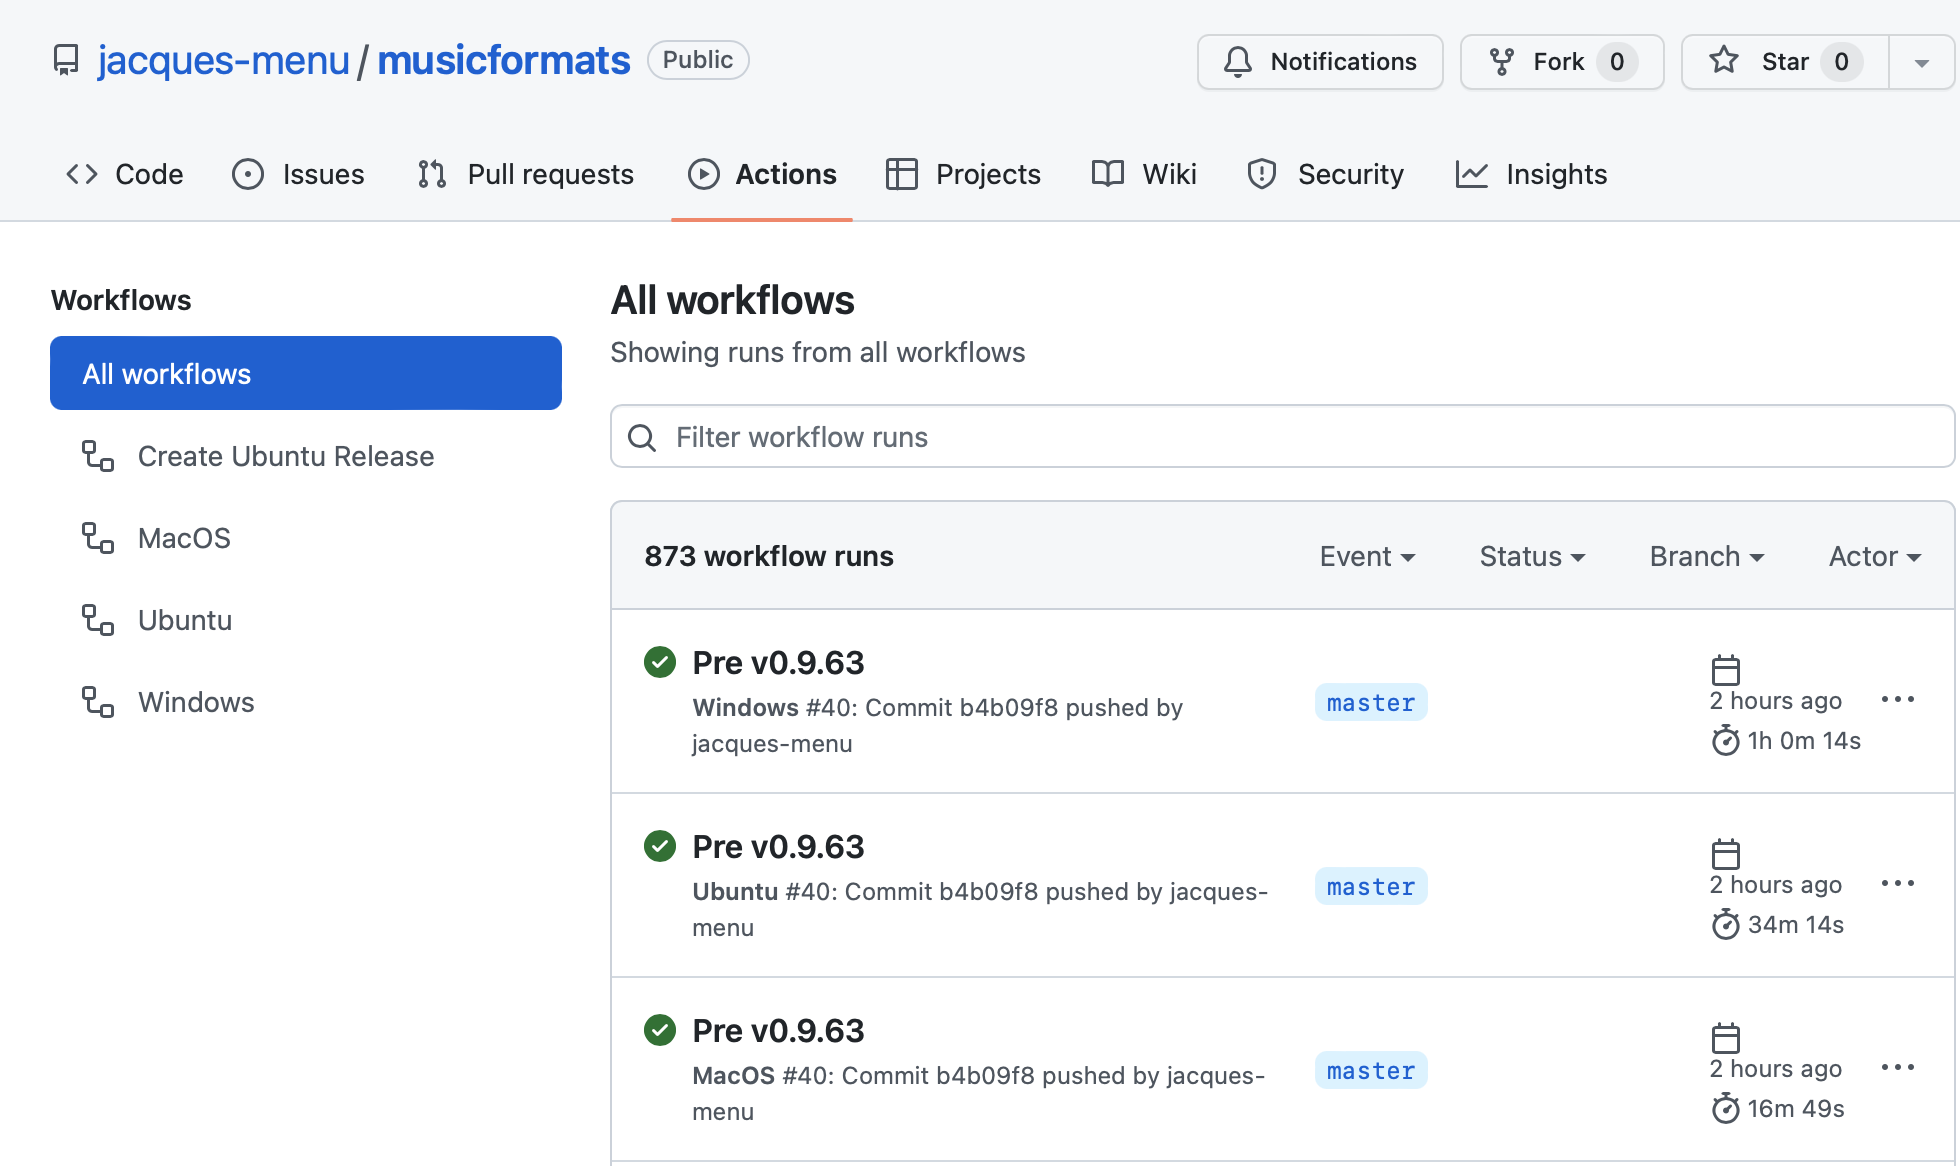
\includegraphics[scale=0.5]{../graphics/SuccessfulActions.png}


\item when that is the case, download each of the three resulting \code{musicformats-*-distrib} archives locally in turn:\\
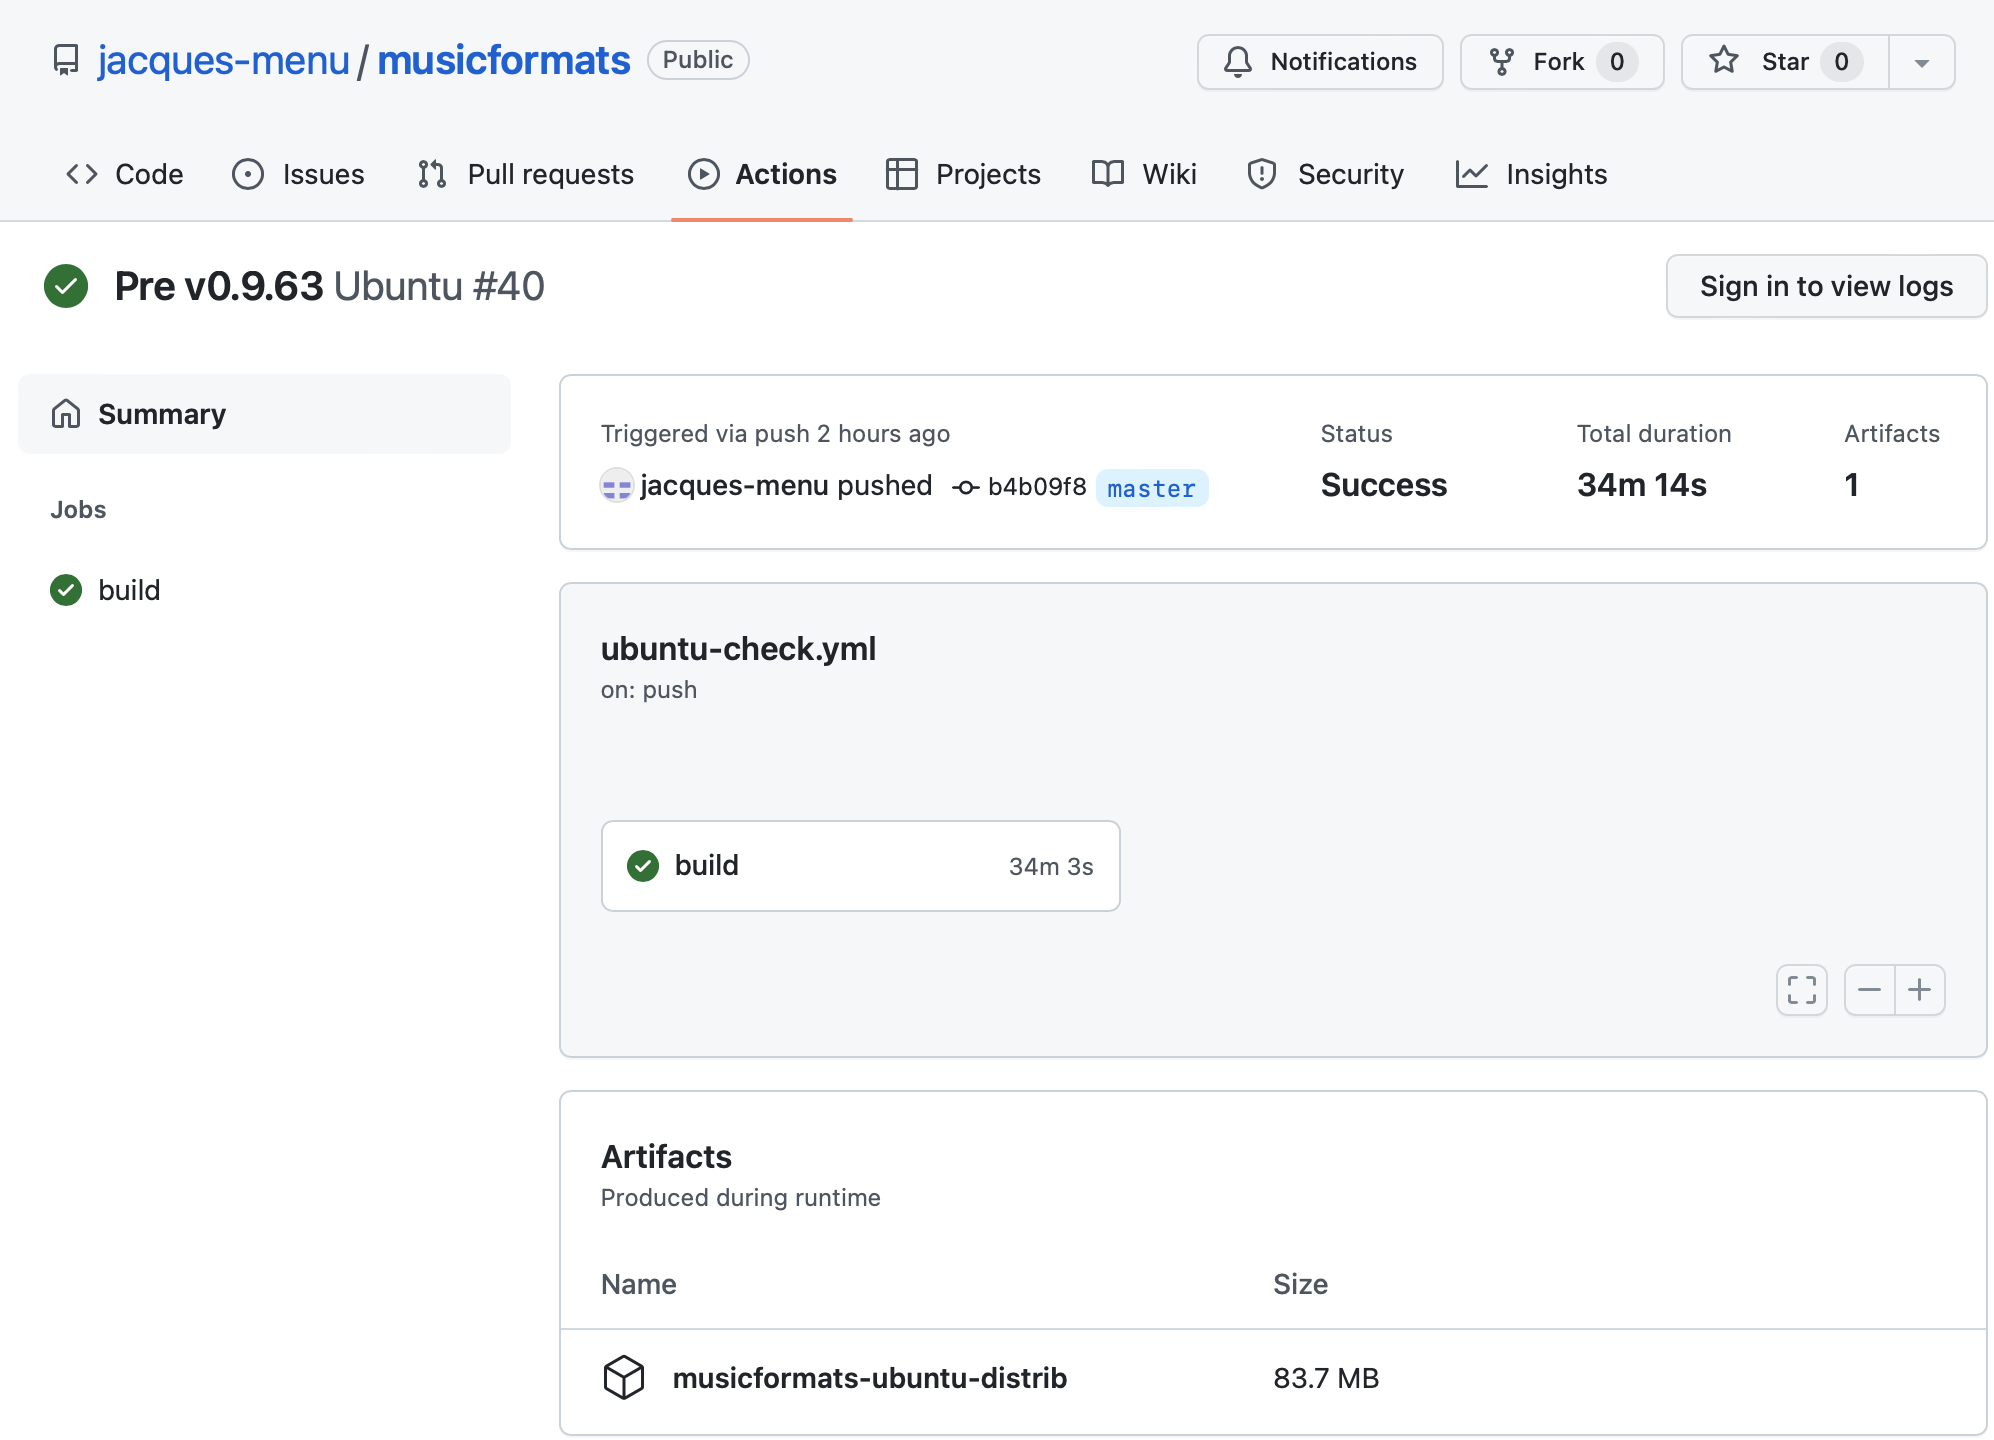
\includegraphics[scale=0.5]{../graphics/DownloadDistribution.png}

On this authors's machine, they go to \code{\$\{HOME\}/Downloads}:
\begin{lstlisting}[language=Terminal]
jacquesmenu@macmini: ~/Downloads > ls -sal musicformats-*-distrib
musicformats-macos-distrib:
total 8
0 drwx------@  5 jacquesmenu  staff  160 Jun  9 11:44 .
0 drwx------+ 28 jacquesmenu  staff  896 Jun  9 11:44 ..
8 -rw-r--r--@  1 jacquesmenu  staff    6 Jun  9 07:40 MusicFormatsVersionNumber.txt
0 drwxr-xr-x@  3 jacquesmenu  staff   96 Jun  9 11:44 build
0 drwxr-xr-x@  4 jacquesmenu  staff  128 Jun  9 11:44 documentation

musicformats-ubuntu-distrib:
total 8
0 drwx------@  5 jacquesmenu  staff  160 Jun  9 11:44 .
0 drwx------+ 28 jacquesmenu  staff  896 Jun  9 11:44 ..
8 -rw-r--r--@  1 jacquesmenu  staff    6 Jun  9 07:57 MusicFormatsVersionNumber.txt
0 drwxr-xr-x@  4 jacquesmenu  staff  128 Jun  9 11:44 build
0 drwxr-xr-x@  4 jacquesmenu  staff  128 Jun  9 11:44 documentation

musicformats-windows-distrib:
total 8
0 drwx------@  5 jacquesmenu  staff  160 Jun  9 11:43 .
0 drwx------+ 28 jacquesmenu  staff  896 Jun  9 11:44 ..
8 -rw-r--r--@  1 jacquesmenu  staff    6 Jun  9 08:14 MusicFormatsVersionNumber.txt
0 drwxr-xr-x@  4 jacquesmenu  staff  128 Jun  9 11:43 build
0 drwxr-xr-x@  4 jacquesmenu  staff  128 Jun  9 11:43 documentation
\end{lstlisting}


\item create the releases in the local \mf\ \repo\ clone:
\begin{lstlisting}[language=TerminalSmall]
jacquesmenu@macmini: ~/musicformats-git-dev > scripts/MakeMusicFormatsDistributions.bash
... ... ...
----------------------------------------------
==> final distrib contents:
----------------------------------------------

  4368 -rw-r--r--  1 jacquesmenu  staff   2234811 Jun  9 11:47 /Users/jacquesmenu/musicformats-git-dev/distrib/MusicFormatsForWindows.zip
 35312 -rw-r--r--  1 jacquesmenu  staff  18076799 Jun  9 11:47 /Users/jacquesmenu/musicformats-git-dev/distrib/MusicFormatsForUbuntu.zip
127824 -rw-r--r--  1 jacquesmenu  staff  65442854 Jun  9 11:47 /Users/jacquesmenu/musicformats-git-dev/distrib/MusicFormatsForMacOS.zip
  1712 -rw-r--r--@ 1 jacquesmenu  staff    872863 Jun  9 07:40 /Users/jacquesmenu/musicformats-git-dev/distrib/IntroductionToMusicXML.pdf
  5328 -rw-r--r--@ 1 jacquesmenu  staff   2724130 Jun  9 07:40 /Users/jacquesmenu/musicformats-git-dev/distrib/MusicFormatsUserGuide.pdf
     8 -rw-r--r--@ 1 jacquesmenu  staff         6 Jun  9 07:40 /Users/jacquesmenu/musicformats-git-dev/distrib/MusicFormatsVersionNumber.txt

/Users/jacquesmenu/musicformats-git-dev/distrib/MusicFormatsForWindows:
total 8
0 drwxr-xr-x  14 jacquesmenu  staff  448 Jun  9 11:47 ..
0 drwxr-xr-x   5 jacquesmenu  staff  160 Jun  9 11:47 .
0 drwxr-xr-x@  4 jacquesmenu  staff  128 Jun  9 11:43 lib
0 drwxr-xr-x@ 26 jacquesmenu  staff  832 Jun  9 11:43 bin
8 -rw-r--r--@  1 jacquesmenu  staff    6 Jun  9 08:14 MusicFormatsVersionNumber.txt

/Users/jacquesmenu/musicformats-git-dev/distrib/MusicFormatsForUbuntu:
total 8
0 drwxr-xr-x  14 jacquesmenu  staff  448 Jun  9 11:47 ..
0 drwxr-xr-x   5 jacquesmenu  staff  160 Jun  9 11:47 .
0 drwxr-xr-x@  4 jacquesmenu  staff  128 Jun  9 11:44 lib
0 drwxr-xr-x@ 26 jacquesmenu  staff  832 Jun  9 11:44 bin
8 -rw-r--r--@  1 jacquesmenu  staff    6 Jun  9 07:57 MusicFormatsVersionNumber.txt

/Users/jacquesmenu/musicformats-git-dev/distrib/MusicFormatsForMacOS:
total 8
0 drwxr-xr-x  14 jacquesmenu  staff  448 Jun  9 11:47 ..
0 drwxr-xr-x   4 jacquesmenu  staff  128 Jun  9 11:47 .
0 drwxr-xr-x@ 26 jacquesmenu  staff  832 Jun  9 07:40 bin
8 -rw-r--r--@  1 jacquesmenu  staff    6 Jun  9 07:40 MusicFormatsVersionNumber.txt
\end{lstlisting}

Now, the local \masterBranch\ contains the release files of itself:
\begin{lstlisting}[language=TerminalSmall]
jacquesmenu@macmini: ~/musicformats-git-dev/distrib > ls -al
total 174552
drwxr-xr-x  14 jacquesmenu  staff       448 Jun  9 11:47 .
drwxr-xr-x  29 jacquesmenu  staff       928 Jun  9 09:13 ..
-rw-r--r--@  1 jacquesmenu  staff    872863 Jun  9 07:40 IntroductionToMusicXML.pdf
drwxr-xr-x   4 jacquesmenu  staff       128 Jun  9 11:47 MusicFormatsForMacOS
-rw-r--r--   1 jacquesmenu  staff  65442854 Jun  9 11:47 MusicFormatsForMacOS.zip
drwxr-xr-x   5 jacquesmenu  staff       160 Jun  9 11:47 MusicFormatsForUbuntu
-rw-r--r--   1 jacquesmenu  staff  18076799 Jun  9 11:47 MusicFormatsForUbuntu.zip
drwxr-xr-x   5 jacquesmenu  staff       160 Jun  9 11:47 MusicFormatsForWindows
-rw-r--r--   1 jacquesmenu  staff   2234811 Jun  9 11:47 MusicFormatsForWindows.zip
-rw-r--r--@  1 jacquesmenu  staff   2724130 Jun  9 07:40 MusicFormatsUserGuide.pdf
-rw-r--r--@  1 jacquesmenu  staff         6 Jun  9 07:40 MusicFormatsVersionNumber.txt
drwx------@  5 jacquesmenu  staff       160 Jun  9 11:44 musicformats-macos-distrib
drwx------@  5 jacquesmenu  staff       160 Jun  9 11:44 musicformats-ubuntu-distrib
drwx------@  5 jacquesmenu  staff       160 Jun  9 11:43 musicformats-windows-distrib
\end{lstlisting}


\item \MainIt{commit and push again} with the new version name, no 'Pre' this time, in the \code{-m "\dots~\dots~\dots"} message, such as:
\begin{lstlisting}[language=Terminal]
jacquesmenu@macmini: ~/musicformats-git-dev > git commit -m "v0.9.63" -a

jacquesmenu@macmini: ~/musicformats-git-dev > git push
\end{lstlisting}


\item create the new version \branch\ locally and remotely:
\begin{lstlisting}[language=Terminal]
jacquesmenu@macmini: ~/musicformats-git-dev > git push --set-upstream origin v0.9.63
Total 0 (delta 0), reused 0 (delta 0), pack-reused 0
remote: 
remote: Create a pull request for 'v0.9.63' on GitHub by visiting:
remote:      https://github.com/jacques-menu/musicformats/pull/new/v0.9.63
remote: 
To https://github.com/jacques-menu/musicformats.git
 * [new branch]      v0.9.63 -> v0.9.63
branch 'v0.9.63' set up to track 'origin/v0.9.63'.

jacquesmenu@macmini: ~/musicformats-git-dev > git branch -r
  origin/HEAD -> origin/master
  origin/gh-pages
  origin/master
  origin/v0.9.60
  origin/v0.9.61
  origin/v0.9.62
  origin/v0.9.63
  
jacquesmenu@macmini: ~/musicformats-git-dev > git branch
* master
  v0.9.63
\end{lstlisting}


\item create a new version number and date, for example:
\begin{lstlisting}[language=TerminalSmall]
jacquesmenu@macmini: ~/musicformats-git-dev > scripts/SetMusicFormatsVersionNumber. bash 0.9.64
-bash: scripts/SetMusicFormatsVersionNumber.: No such file or directory
jacquesmenu@macmini: ~/musicformats-git-dev > scripts/SetMusicFormatsVersionNumber.bash 0.9.64
==> PWD is:
/Users/jacquesmenu/musicformats-git-dev

==> Writing MusicFormats version number 0.9.64 to MusicFormatsVersionNumber.txt

8 -rw-r--r--  1 jacquesmenu  staff  6 Jun  9 12:14:57 2022 MusicFormatsVersionNumber.txt
0.9.64
==> PWD is:
/Users/jacquesmenu/musicformats-git-dev/src

==> Writing MusicFormats version number 0.9.64 to MusicFormatsVersionNumber.h

8 -rw-r--r--  1 jacquesmenu  staff  45 Jun  9 12:14:57 2022 MusicFormatsVersionNumber.h
#define MUSICFORMATS_VERSION_NUMBER "0.9.64"
\end{lstlisting}

\begin{lstlisting}[language=Terminal]
jacquesmenu@macmini: ~/musicformats-git-dev > scripts/SetMusicFormatsVersionDate.bash "June 9, 2022"
==> PWD is:
/Users/jacquesmenu/musicformats-git-dev

==> Writing MusicFormats version date June 9, 2022 to MusicFormatsVersionDate.txt

8 -rw-r--r--  1 jacquesmenu  staff  13 Jun  9 12:15:52 2022 MusicFormatsVersionDate.txt
June 9, 2022

==> PWD is:
/Users/jacquesmenu/musicformats-git-dev/src

==> Writing MusicFormats version date June 9, 2022 to MusicFormatsVersionDate.h

8 -rw-r--r--  1 jacquesmenu  staff  49 Jun  9 12:15:52 2022 MusicFormatsVersionDate.h
#define MUSICFORMATS_VERSION_DATE "June 9, 2022"
\end{lstlisting}

Check the result with:
\begin{lstlisting}[language=Terminal]
jacquesmenu@macmini: ~/musicformats-git-dev > scripts/ShowMusicFormatsVersion.bash 
Version number:
0.9.64Version date:
June 9, 2022
\end{lstlisting}

\end{enumerate}
